\chapter{Progress}\label{C:ex}


\section{Geological Background}
During the mid-semester break there was a trip to Nelson as part of an introductory field geology paper, ESCI-241. The relevancy of this exercise was to conceptualize the gathered data the various AI techniques would be working upon. This trip gave a lot of insight into understanding the scale of various stratigraphic layers and their composition. It also brought up a number of points that are out of scope for this project but will need addressing before any of the proposed solutions are industry ready.


The main point being that the contact between layers is rarely horizontal. Over an aperture distance of 20-30 meters the reading of these contacts would become distorted, producing data that is hard to accurately model using the proposed AI solutions. This problem exists within the current human operated simplex method but an experienced technician will have relevant structural background to understand these features that the AI solutions would find hard to model.  This leads further credence to the need to fix a number of simplifications used within previous work.


Another generalization that this work and previous work uses is that there are only ever two layers. This excursion demonstrated that while there are often only one or two layers that would have an effect on the surface layer, the current work still does not support this variance. Examples of a number of sites that had more than 2 layers were also witnessed. This is the easier of the two generalization to amend. 
\section{Implementation of Existing Work}
A major achieved milestone was the handover of the existing work and the familiarization with the system to the point where the past experiments can be repeated. This has involved updating the existing implementation to work on the updated ECS system that is now running Java 7 rather than 6. A refactoring of several duplicated classes has occurred to make the system more readable and allow the extraction of the libCPS library. Scripts have been successfully written to allow batch testing and experiment duplication over the grid.

\section{Benchmark Data Acquisition}

In order to successfully compare the different AI methods a substantial amount of data needs to be collected. The data that Aaron collected from the PLGP is not sufficient to fairly contrast the other techniques against. Due to time constraints and the slow nature of libCPS, generations were limited to 50. The oscillation phenomena Aaron experienced may be reducible using a larger number of generations \cite{scoble1}.


Aaron acknowledges his work as a proof of concept and does not provide rigorous testing of the ESPAC technique. So a new step within the project has to be to gather a set of statistically strong data. There were a number of decisions related to the configuration of these experiments that needed to be made. As the best operational conditions have yet to be determined for the PLGP implementation additional experiments to contrast a number of different run configurations need to occur. The next section details the following experiments that have been run or are in the process of running to fulfill this.

\section{PLGP Results}

Still waiting on more grid results before the data can be empirically evaluated. Once these results are in a study of the data using both Student's paired sample t-tests and Wilcoxon rank-sum test will be conducted.



\subsection{Population 100 with 80 Generations}
This was the first experiment to have a significant number of runs, 30, on the grid. The numbers were chosen with a focus on determining the speed at which the program executed. These runs took on average 22 hours to complete.
\\\\
The graphs in Figure 3.1 show a cross section of the data collected for the PLGP running with a population of 100 with 80 generations. It is expected that the variance is due to the small population size and that decreasing the number of generations by half will have little effect on the fitness.


\begin{figure}[h]
{\begin{center}
\begin{tabular}{ll}
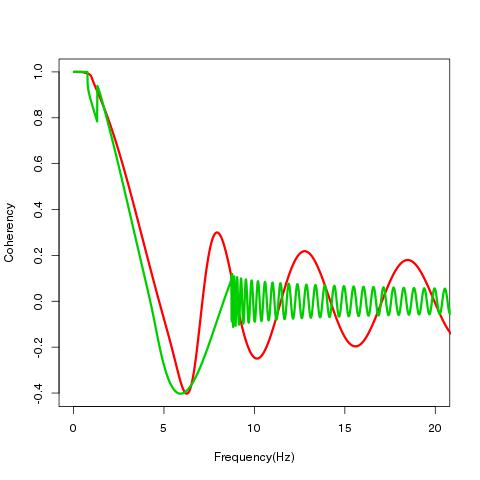
\includegraphics[width=80mm]{pop1003.jpg} & 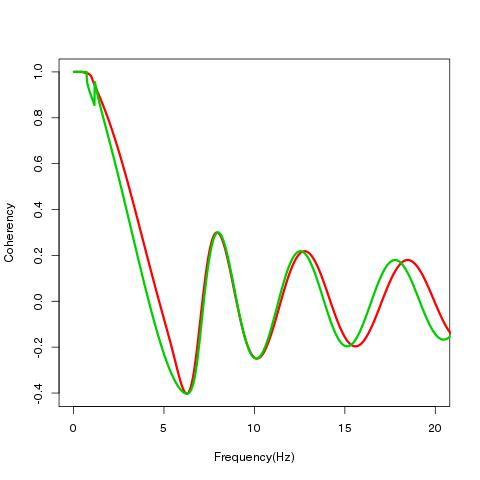
\includegraphics[width=80mm]{pop1002.jpg}
\end{tabular}
\caption{Two graphs highlighting the variance found within 30 runs of the PLGP with a population of 100 and 80 generations}
\end{center}}
\end{figure}
\clearpage

\subsection{Population 100 with 40 Generations}

The purpose of this experiment is to determine the difference found between changing the number of generations over a small population.
\\\\
Results Pending

\subsection{Population 1000 with 40 Generations}
The purpose of this experiment is to determine the difference found between changing the population and to determine the speed of the application. The average run time for these was 4.8 days.
\\\\
The graphs in Figure 3.2 show a cross section of the data collected for the PLGP running with a population of 1000 with 40 generations. The variance seen here is very similar to that seen with a population of 100 and 80 generations. As we proposed that 100 populations with 40 generations would be similar this indicates our smallest set of runs is providing an optimal solution given the current fitness function.



\begin{figure}[h]
{\begin{center}
\begin{tabular}{ll}
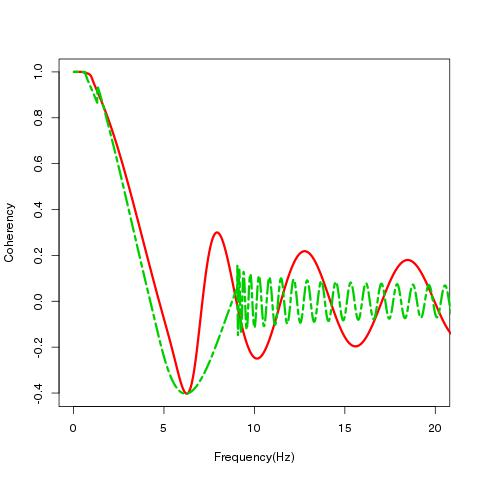
\includegraphics[width=80mm]{pop10001.jpg} & 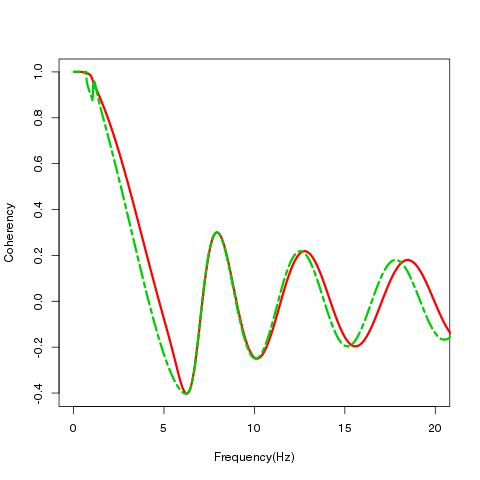
\includegraphics[width=80mm]{pop10003.jpg}
\end{tabular}
\caption{Two graphs highlighting the variance found within 30 runs of the PLGP with a population of 1000 and 40 generations}
\end{center}}
\end{figure}
\subsection{Population 1000 with 80 Generations}
The purpose of this experiment is to satisfy our hypothesis that a population of 1000 with 80 generations will have the same variance and local optimization as a run with a population of 100 with 40 generations.
\\\\
Still waiting on grid results before this hypothesis can be evaluated.



\section{GA Implementation}

A basic GA has been implemented following a number of ECJ tutorials. The purpose of this was to gain an understanding of the library before attempting the full GP. The GA is fairly basic and not suited to the regression problem so out side of this exercise it will not be used or test.

\section{GP Implementation}

Currently just the ECJ tutorial has been implemented. A full implementation of the GP is the next major hurdle that will be accomplished.
